\documentclass[../Article_Model_Parameters.tex]{subfiles}
\graphicspath{{\subfix{../Figures/}}}
\begin{document}
	
	\label{CH: Results}
	
	This work investigates the influence of inlet temperature, pressure, and mass flow rate on the state space and the extraction yield. The process model and parameters have been discussed in {\color{red}article 1}. The process model was calibrated on set of experiments obtained at different operating conditions, $40^\circ C$ - $50^\circ C$ and 200 bar - 300 bar. The sensitivity analysis has been performed under the assumption that the system operates are $45^\circ C$, 250 bar and 0.4 l/min, which is the middle of the range of operating conditions.
	
	\subsection{Flow-rate}
	
	The increase in the mass-flow rate affects the whole system simultaneously in the spatial direction. The change in mass flow-rate makes the fluid move faster and does not directly affect the thermodynamic state of the fluid. As a result, Figure \ref{fig:Sensitivty_F_P} shows no change in pressure during the simulation. 
    
    \begin{figure}[h!]
    	\centering
    	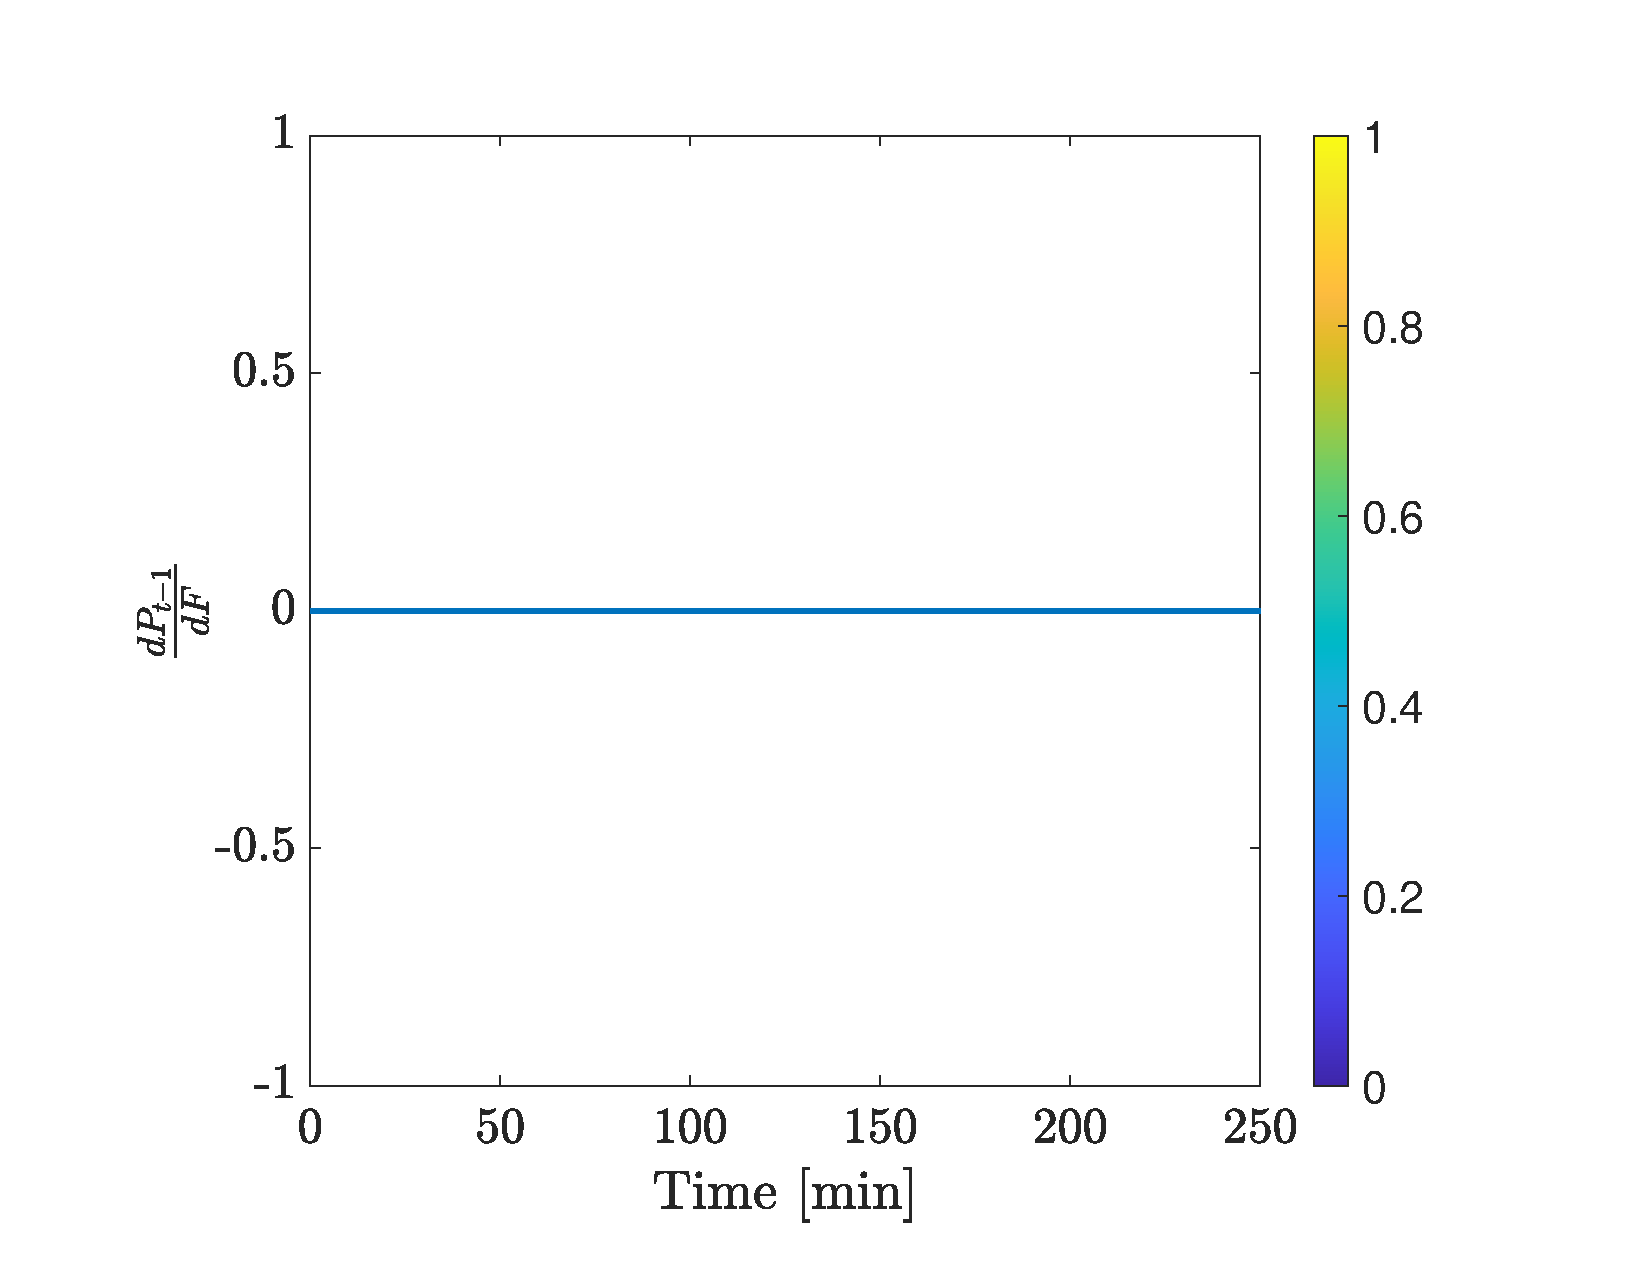
\includegraphics[trim = 1.5cm 1cm 0.0cm 1.0cm,clip,width=\columnwidth]{/Results_sensitivity/P_F.pdf}
    	\caption{The effect of $F$ change on $P$}
    	\label{fig:Sensitivty_F_P}
    \end{figure}
    
    A flow rate change is defined by the spatial derivative $\frac{\partial \left( {\color{orange}\rho_f}{\color{blue}h} A_f v \right)}{\partial {\color{blue}z}}$. The consequence of Equation \ref{EQ:Velocity} is the instantaneous change of the velocity field in the system, which means that the spatial derivative equals zero. It's important to note that ${\color{blue}h}$ represents enthalpy but not total enthalpy, thus excluding kinetic energy contribution. As a consequence of our modelling assumptions, changes in ${\color{blue}h}$ and ${\color{orange}\rho_f}$ only occur in response to direct change in pressure or temperature. As the result, Figure \ref{fig:Sensitivty_F_H} demonstrates no significant deviation.
    
    The flow rate change affects the fluid inside the system, but appropriate boundary conditions must be set. When utilizing Dirichlet boundary conditions, it's crucial to be aware of potential numerical artifacts from the differing methods used to compute them. The system's enthalpy is determined through the time evolution of governing equations, while the inlet's enthalpy depends on the inlet temperature and pressure. A minor numerical mismatch between these values may manifest as an enthalpy difference propagating along the spatial domain. To ensure consistency between the fluid at the inlet and inside the computational domain, this analysis employs Neumann boundary conditions.
        
    \begin{figure}[h!]
    	\centering
    	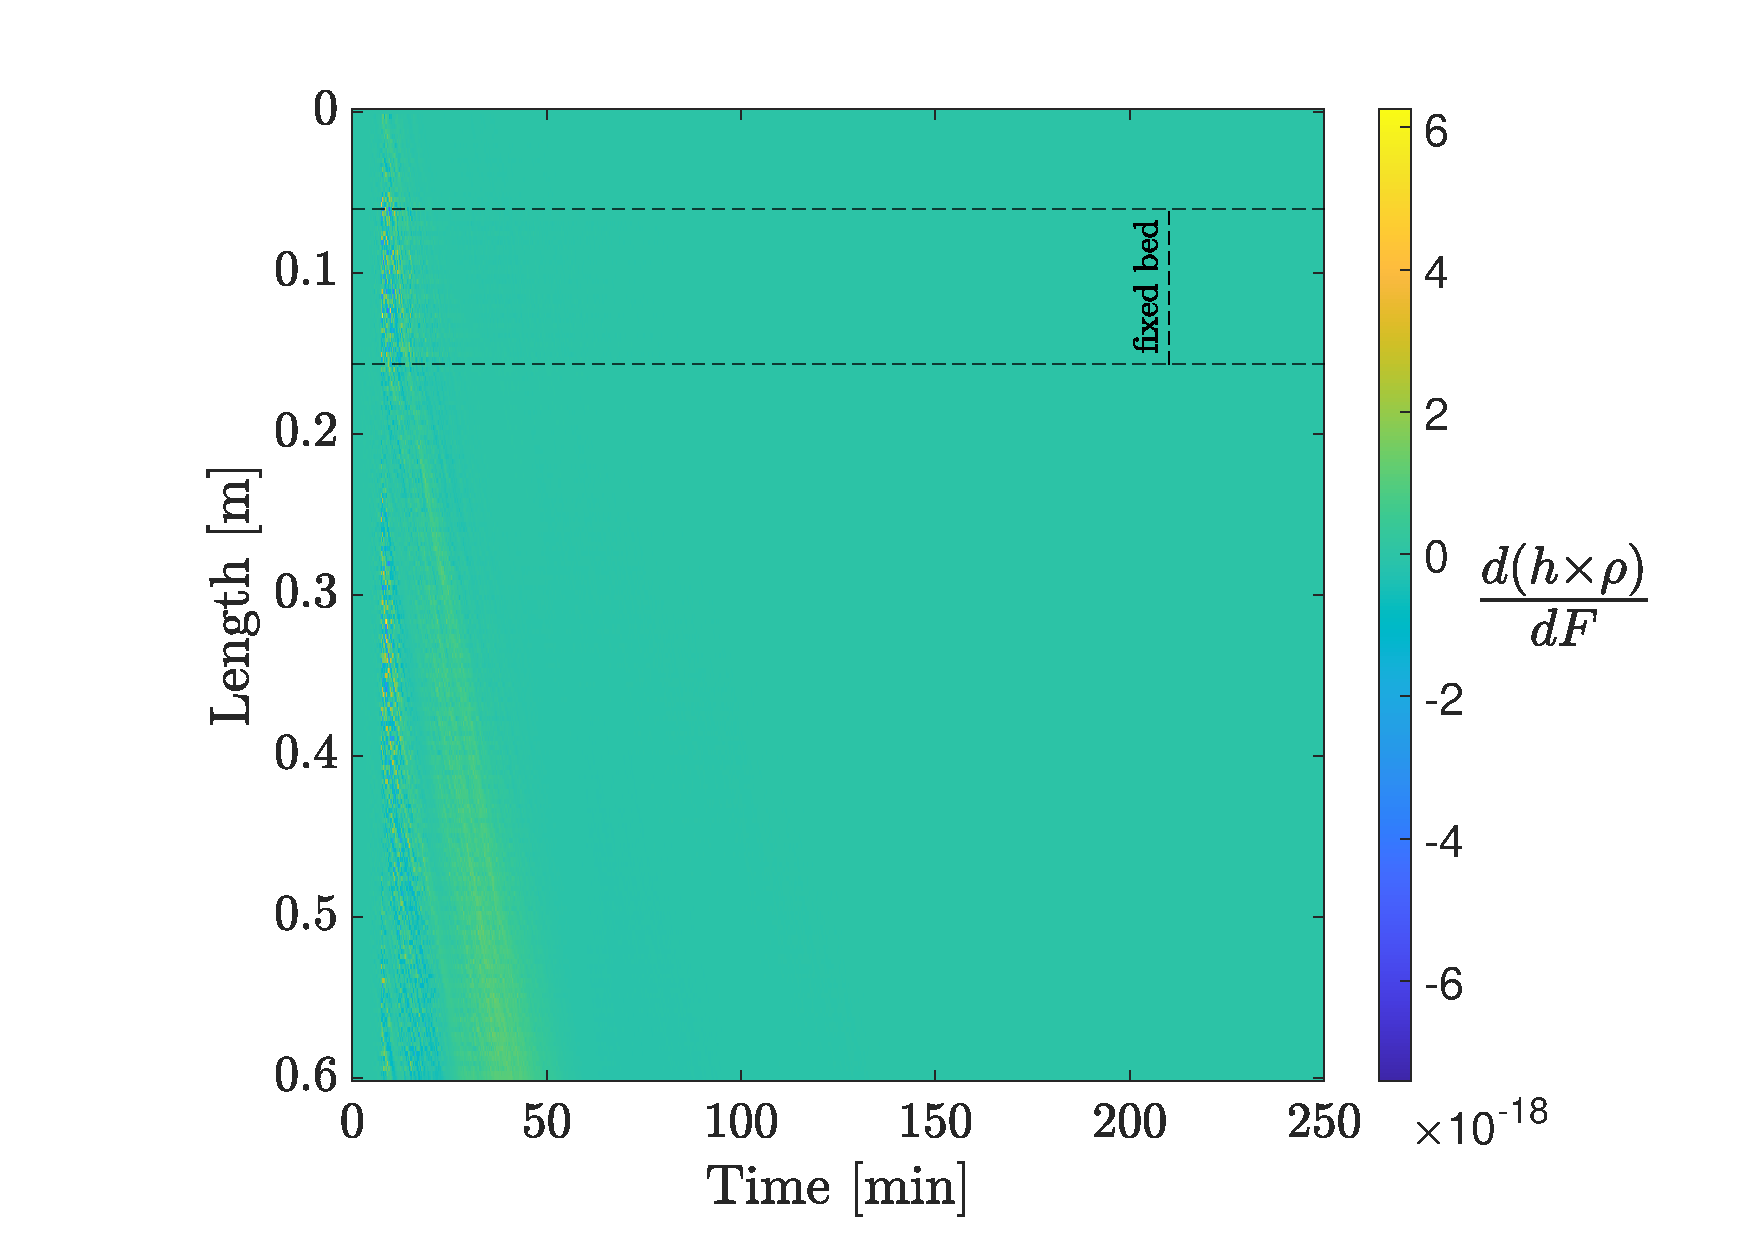
\includegraphics[trim = 1.5cm 1cm 0.0cm 1.0cm,clip,width=\columnwidth]{/Results_sensitivity/H_F.pdf}
    	\caption{The effect of $F$ change on $\rho \times h$}
    	\label{fig:Sensitivty_F_H}
    \end{figure}
   
   An increase in the mass flow rate impacts the concentration gradient and the extraction kinetics as presented in Figure \ref{fig:Sensitivty_F_CS} . At the beginning of the extraction process, changes in the flow rate have a minimal effect on the extraction process, as showed by sensitivities that are close to zero. This is due to the dominance of the high concentration gradient, which leads the extraction kinetic. As time progresses, the increase in the mass flow rate have greater influence on the extraction kinetics, causing the sensitivities to decrease towards their minimum values. Negative sensitivities indicate a faster extraction rate. Over time, the amount of solute in the solid phase decreases, and eventually, the extraction kinetic becomes limited by the concentration gradient. This behavior is represented in the sensitivities, which asymptotically approach zero. The asymptotic movement of sensitivities can be explained by the fact that an increase in the flow rate does not impact the extraction process when all the solute has been removed from the solid phase.
    
    \begin{figure}[h!]
    	\centering
    	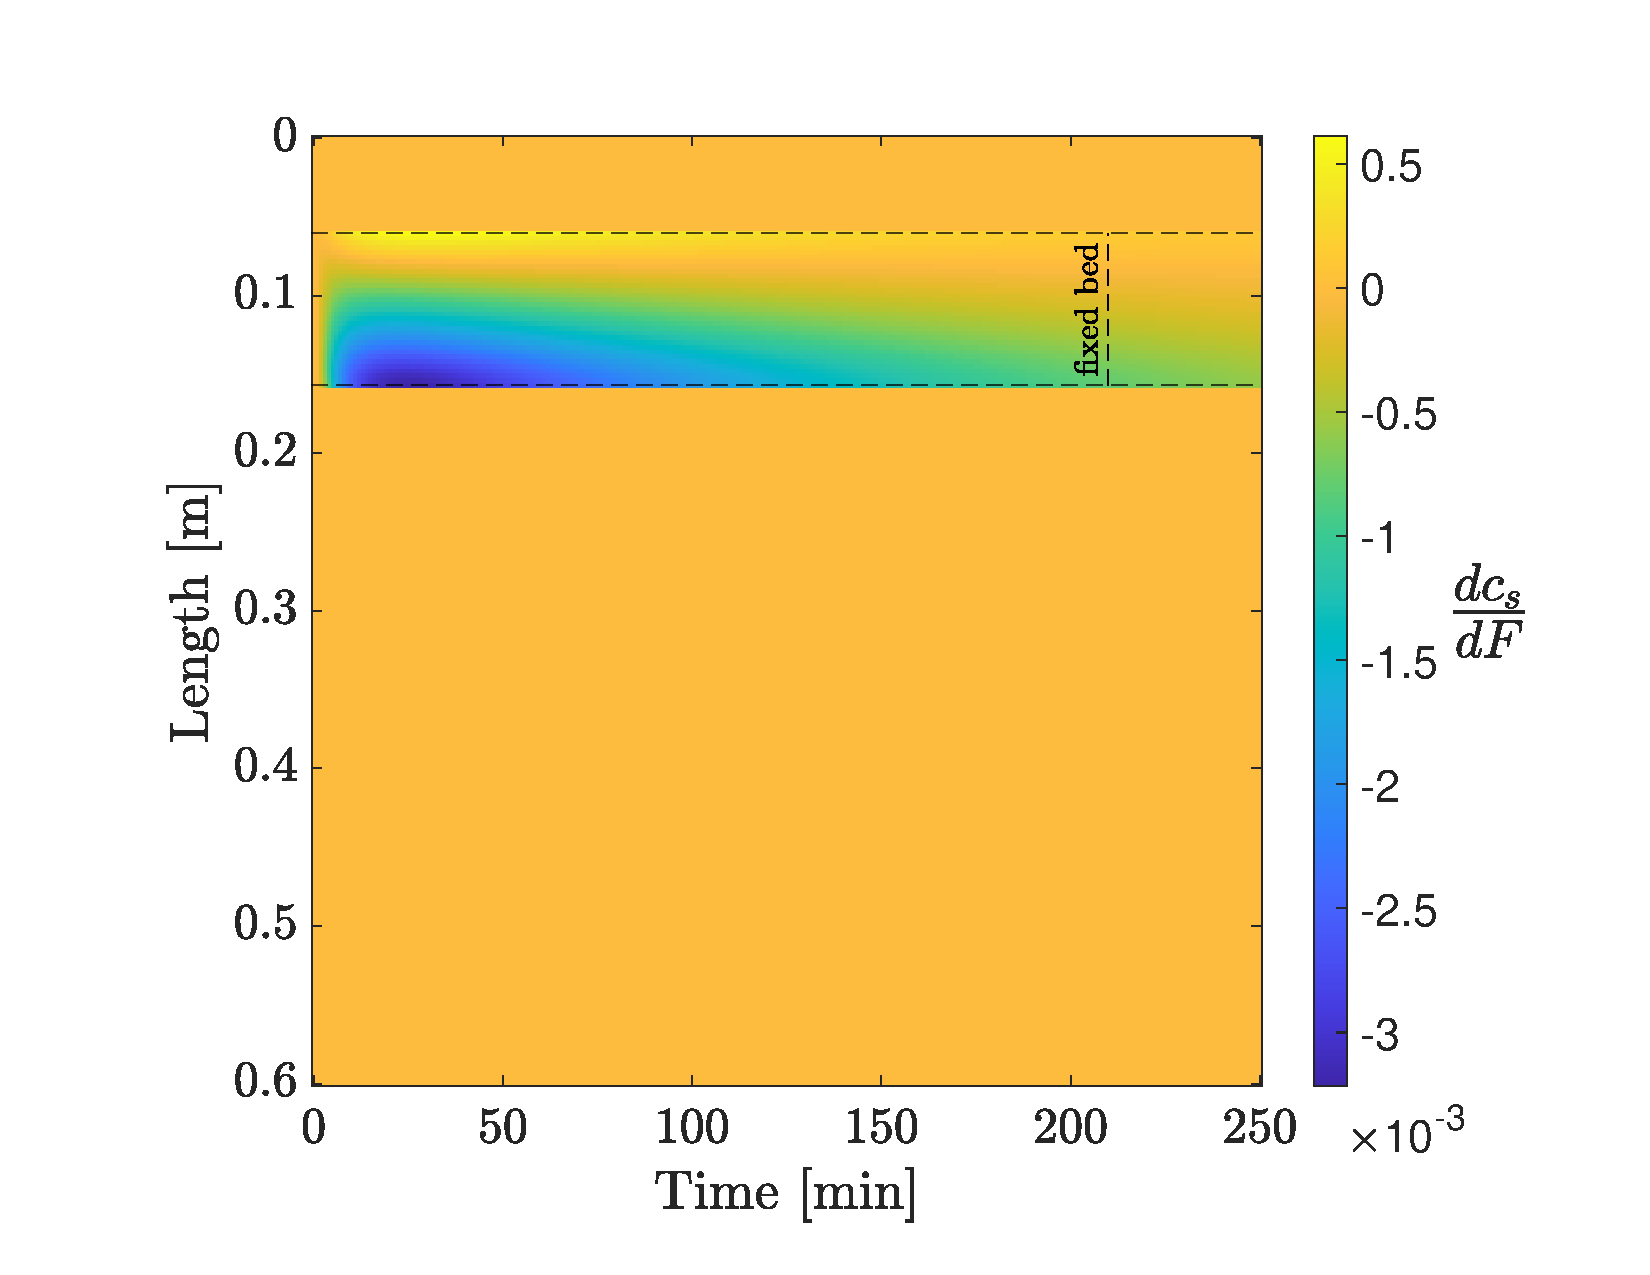
\includegraphics[trim = 1.5cm 1cm 0.0cm 1.0cm,clip,width=\columnwidth]{/Results_sensitivity/CS_F.pdf}
    	\caption{The effect of $F$ change on $C_s$}
    	\label{fig:Sensitivty_F_CS}
    \end{figure}
    
    Figure \ref{fig:Sensitivty_F_CF} illustrates how the concentration of solute in the fluid phase responds to an increase in the flow rate. Initially, sensitivities are close to zero, indicating a minimal system response. The growth in flow rate affects ${\color{blue}C_f}(z,t)$ by increasing the velocity, consequently elevating the concentration gradient. As a result, positive sensitivities emerge within the system, forming a front that progresses in the direction of flow. The positive front indicates that the larger amount of solute moves faster across the system, which leads to faster decrease of the total amount of solute in both phases. This reduced amount of solute in the solid phase restricts the extraction rate due to a diminishment of the concentration gradient. This limitation leads to the formation of a front composed of negative sensitivities, which propagate through the extractor. The negative front indicates that the solute concentration in the fluid phase becomes lower than before the flow rate increment. Eventually, the negative sensitivities asymptotically approach zero.
    
    \begin{figure}[h!]
    	\centering
    	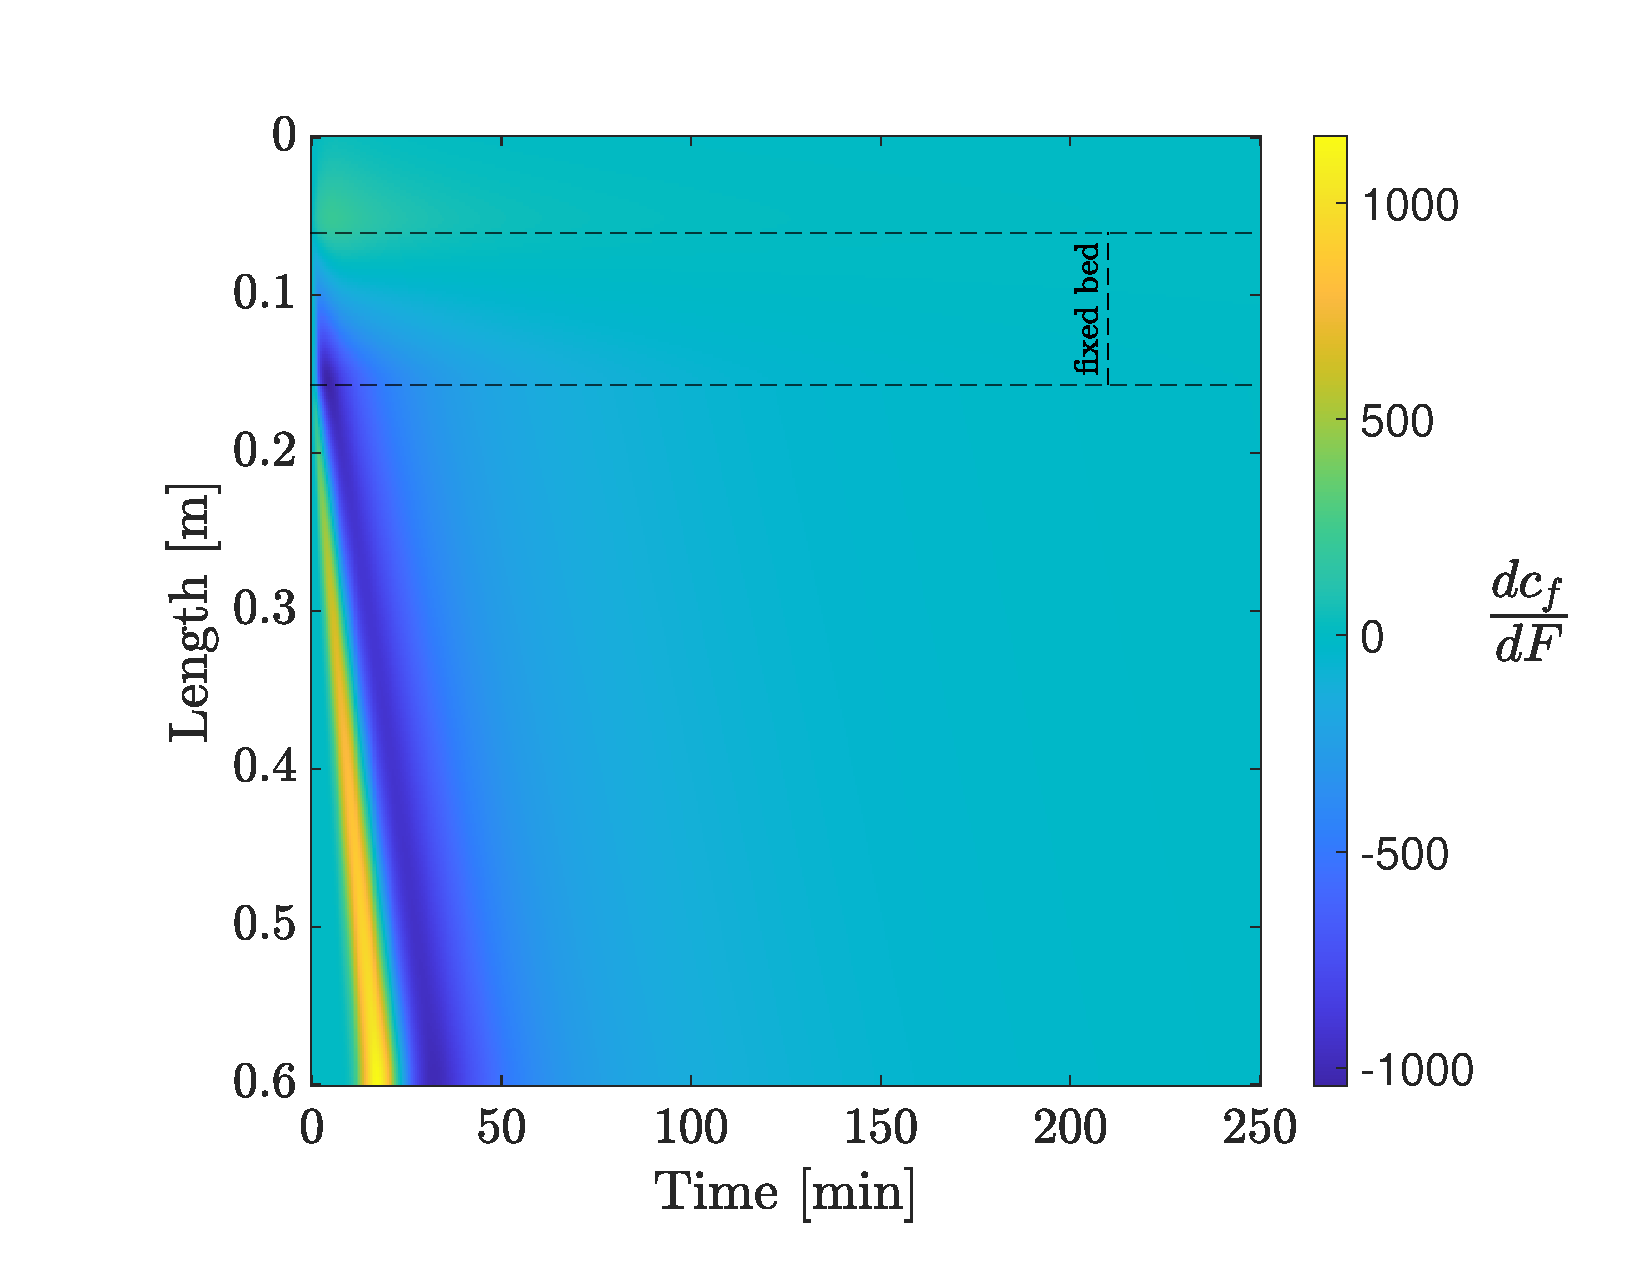
\includegraphics[trim = 1.5cm 1cm 0.0cm 1.0cm,clip,width=\columnwidth]{/Results_sensitivity/CF_F.pdf}
    	\caption{The effect of $F$ change on $C_f$}
    	\label{fig:Sensitivty_F_CF}
    \end{figure}

    Figure \ref{fig:Sensitivty_F_y} illustrates how the increase in flow rate affects the extraction yield. Initially, the sensitivity curve remains flat. This occurs because the fixed bed doesn't occupy the entire volume of the extractor, requiring some time for the fluid to flow through the empty portion of the extractor to reach its outlet. It's only when the solute in the fluid phase reaches the extractor's outlet that we can measure and observe the system response. At this point, $dy/dF$ begins to increase. The positive sensitivity value indicates an improvement in process efficiency, resulting in an increased yield. As time progresses, the sensitivity reaches its maximum and then diminishes due to a decreasing concentration gradient. Eventually, $dy/dF$ asymptotically approaches zero. This happens because the amount of solute in the fluid phase becomes a limiting factor in the extraction process, and the increase in flow rate has a reduced impact on the extraction yield. The simulation time was extended to demonstrate the convergence of $dy/dF$ toward zero.
    
    \begin{figure}[h!]
    	\centering
    	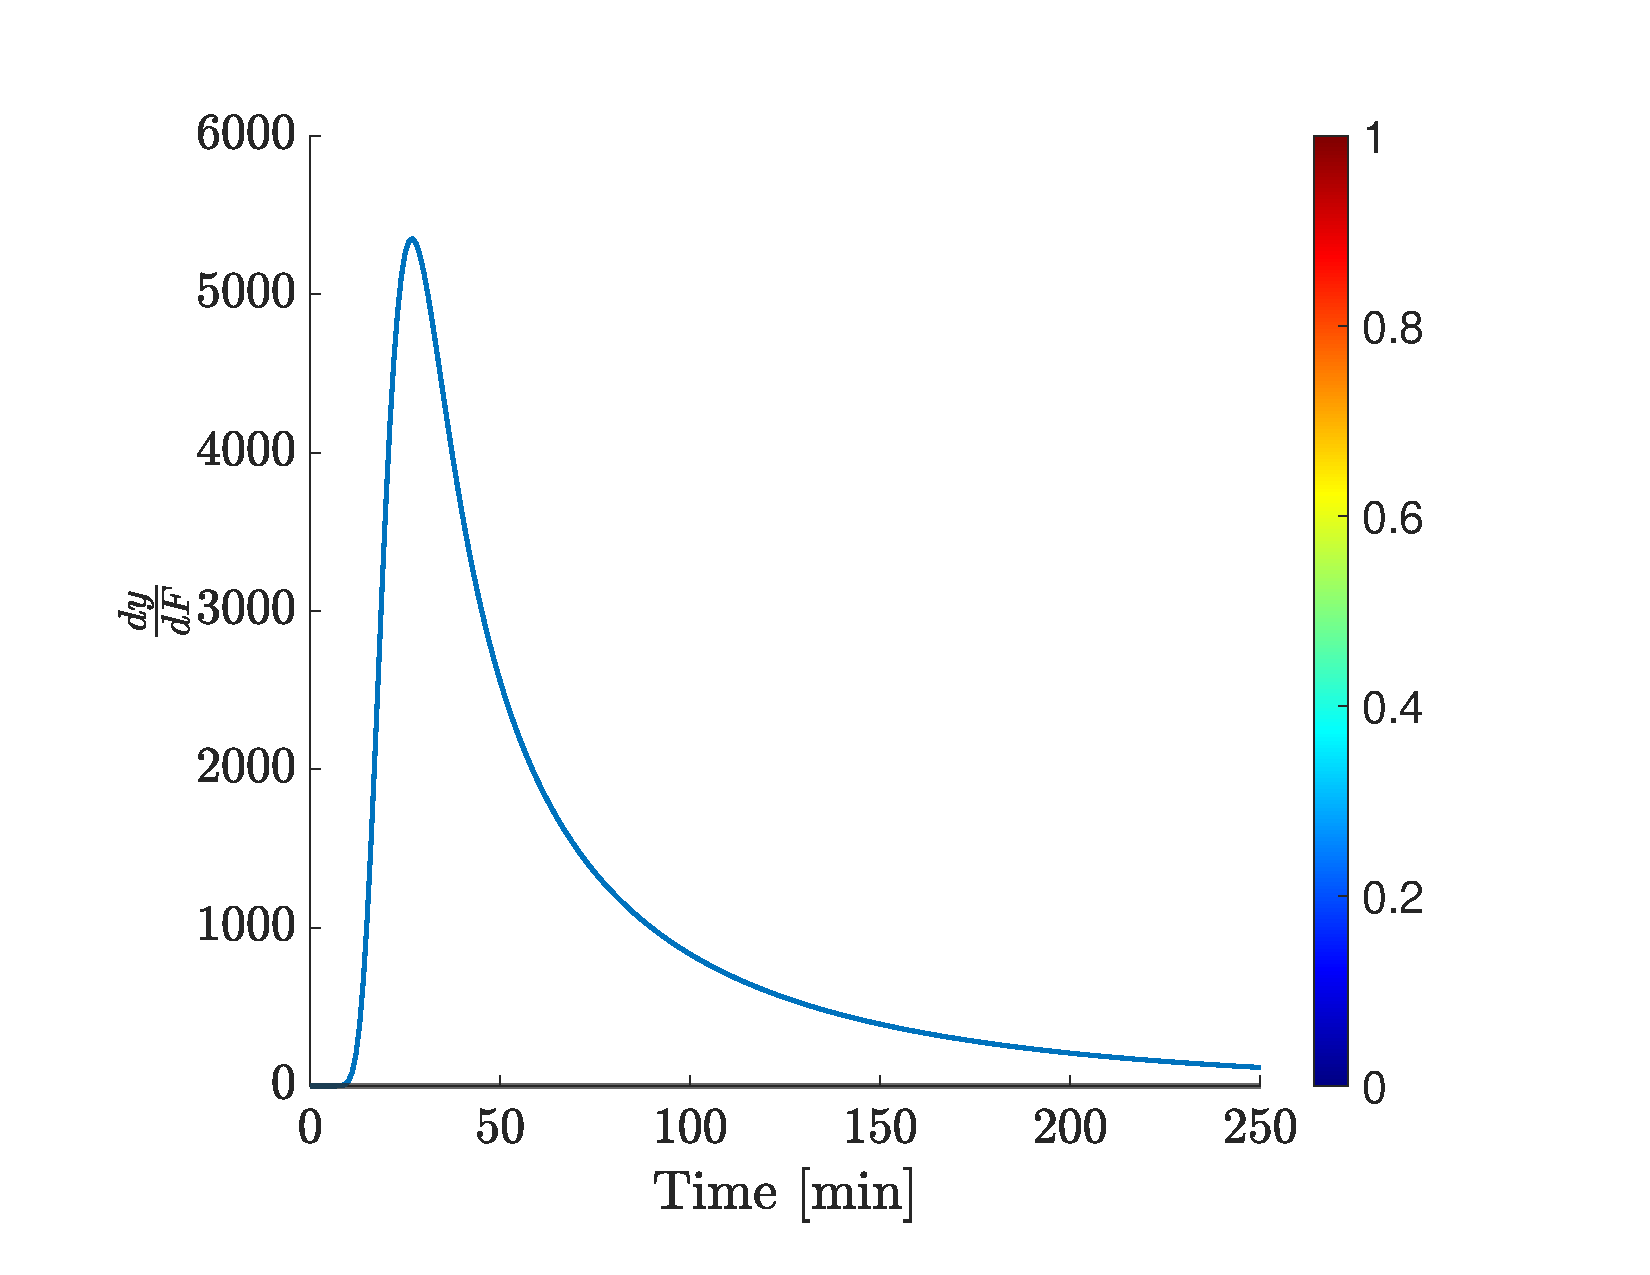
\includegraphics[trim = 1.5cm 1cm 0.0cm 1.0cm,clip,width=\columnwidth]{/Results_sensitivity/Y_F.pdf}
    	\caption{The effect of $F$ change on $y(t)$}
    	\label{fig:Sensitivty_F_y}
    \end{figure}
    
    \subsection{Pressure}
    
    As discussed in Chapter \ref{CH:Governing_equations_chapter}, a small pressure wave propagates at the speed of sound relative to the flow. If the flow velocity is relatively low, all pressure changes are hydrodynamic (resulting from velocity motion) rather than thermodynamic. The Low Mach-number assumption enables instant pressure propagation throughout the system. This assumption allows to consider a single pressure value for the entire system, as all changes occur simultaneously within the machine. Figure \ref{fig:Sensitivty_P_P} illustrates a step function representing the pressure change in the system.
    
    \begin{figure}[h!]
    	\centering
    	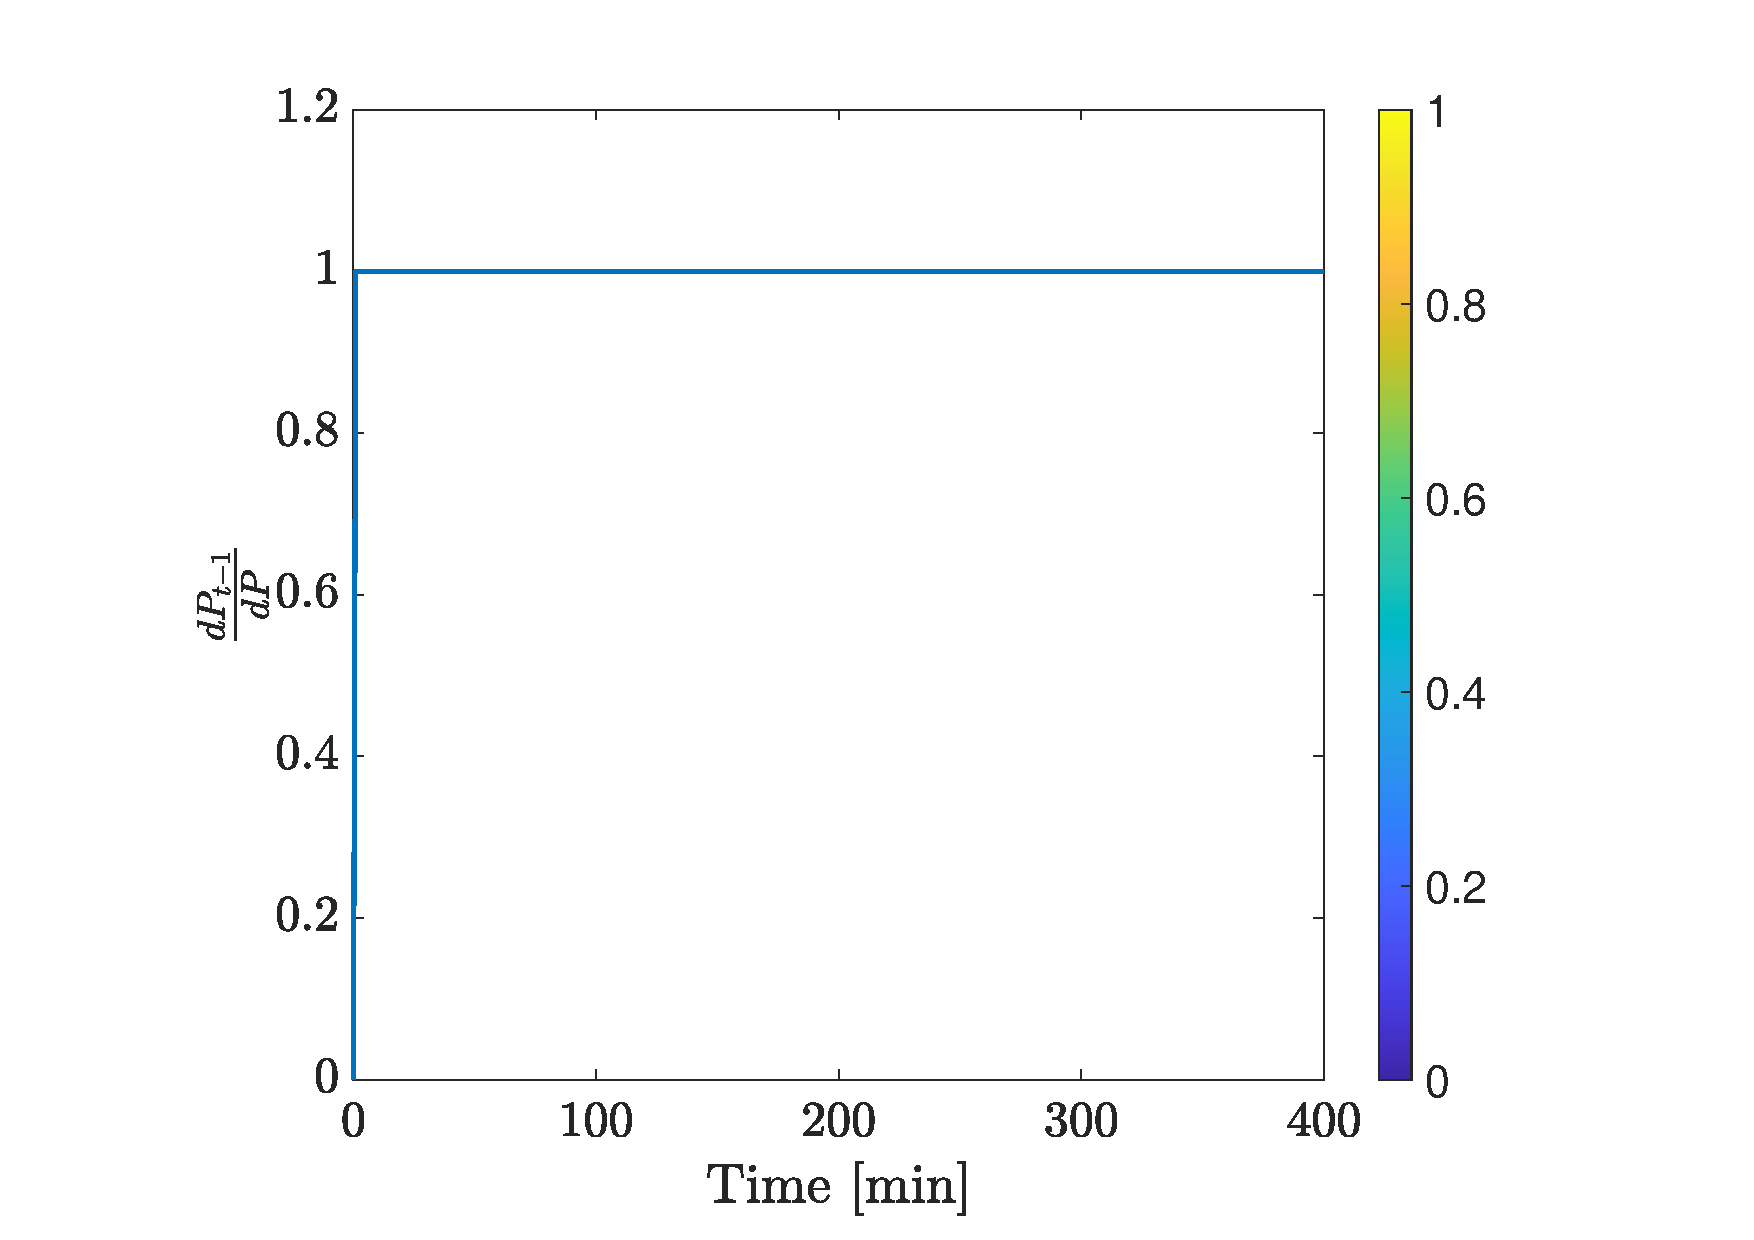
\includegraphics[trim = 1.5cm 1cm 0.0cm 1.0cm,clip,width=\columnwidth]{/Results_sensitivity/P_P.pdf}
    	\caption{The effect of $P$ change on $P$ in the system}
    	\label{fig:Sensitivty_P_P}
    \end{figure}
    
	As a result of the Low Mach-number assumption and the pressure deviation, temperature and density change simultaneously along the system. According to Equation \ref{EQ:Enthalpy_equation}, the pressure change directly affects the quantity $h \times \rho_f$ through $\partial ({\color{blue}P}(t) A_f) / \partial t$, leading to the step change presented in Figure \ref{fig:Sensitivty_P_H}. Depending on the configuration of the system, two cases are possible. Since the total energy in the extractor has changed, there may be a difference between the fluid inside the equipment and the boundary conditions at the inlet. If Dirichlet boundary conditions are applied, the inlet temperature is maintained at the predefined value and may differ from the temperature in the extractor. In such a case, the temperature difference will cause the heat front to propagate through the system. Alternatively, Neumann boundary conditions can be applied to ensure that the temperature inside the extractor matches that at its inlet. In this work, the second approach was chosen.
    
    \begin{figure}[h!]
    	\centering
    	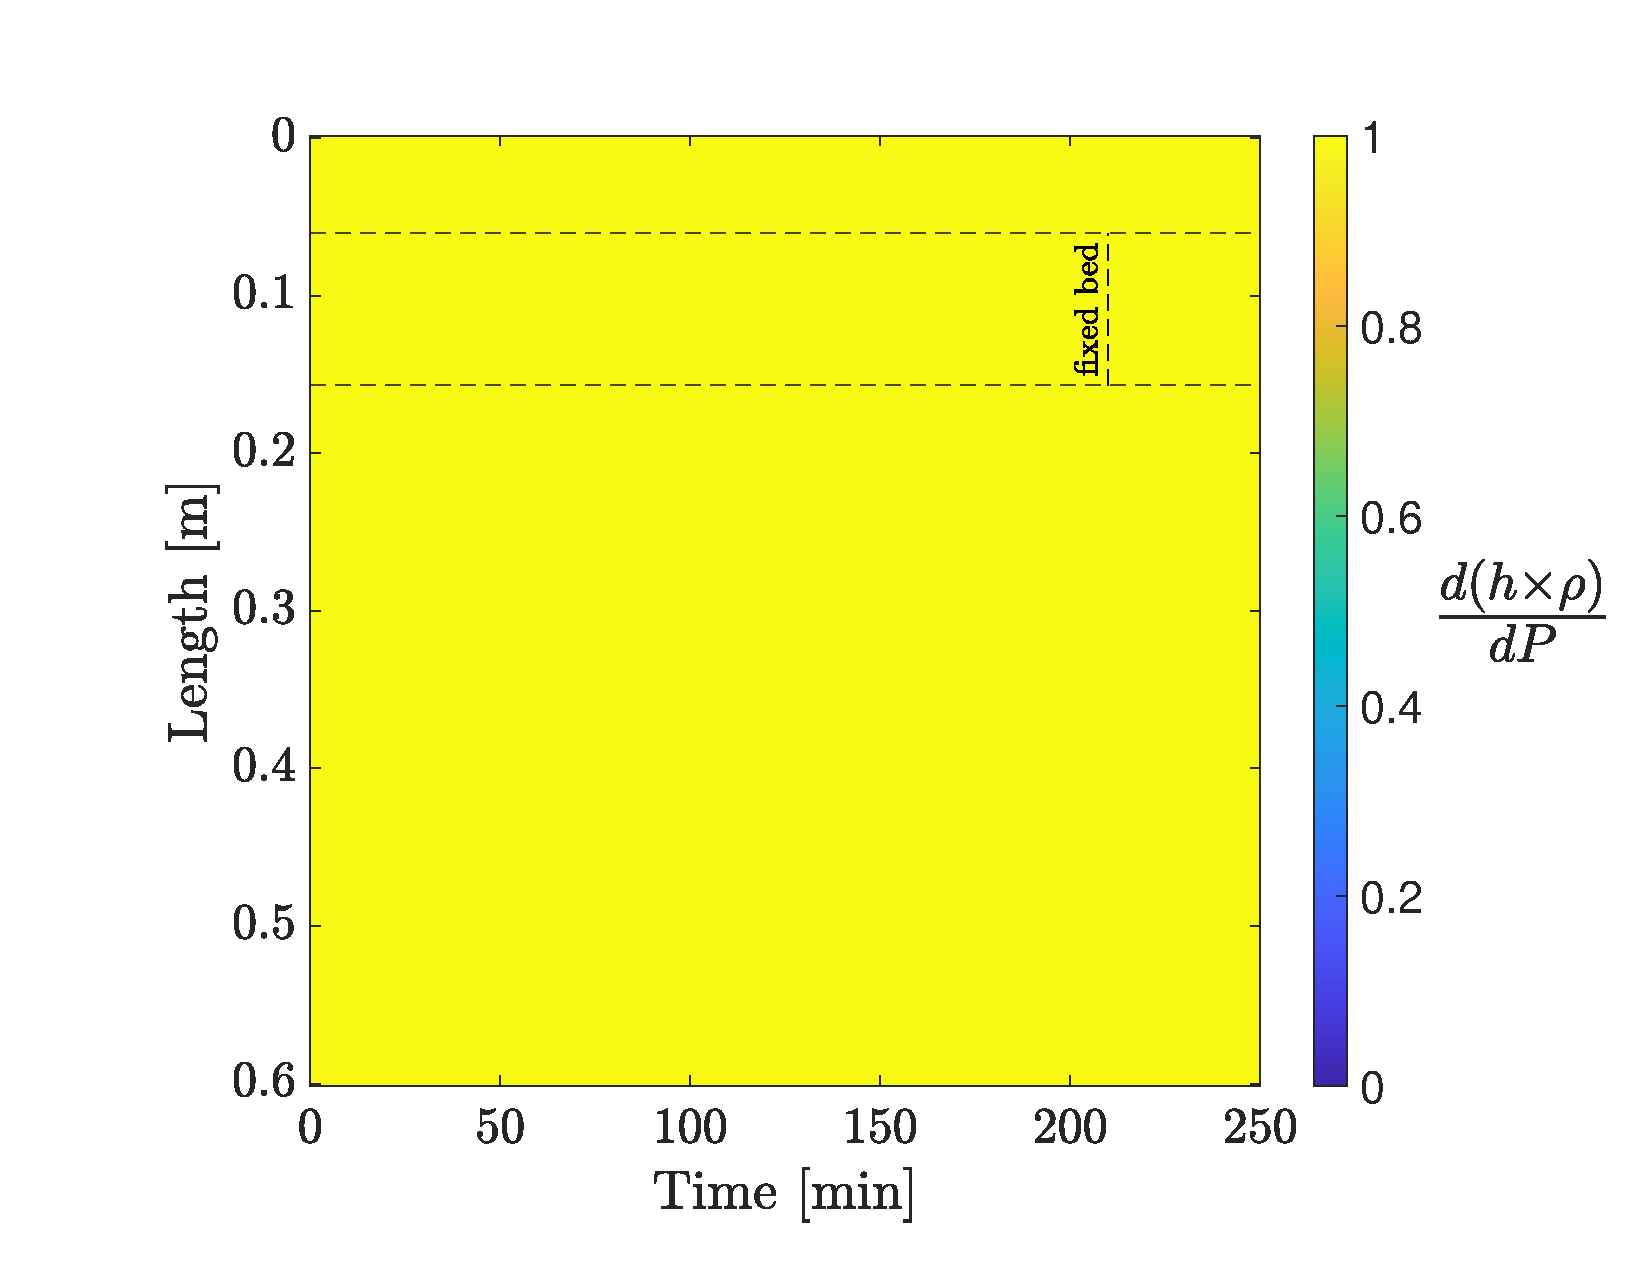
\includegraphics[trim = 1.5cm 1cm 0.0cm 1.0cm,clip,width=\columnwidth]{/Results_sensitivity/H_P.pdf}
    	\caption{The effect of $P$ change on $(h \times \rho_f)$ in the system}
    	\label{fig:Sensitivty_P_H}
    \end{figure}

	The pressure change affects the mass transfer in two ways. As given in Chapter \ref{CH: Continuity}, the velocity is inversely proportional to the density; hence, the higher density of the fluid leads to a lower velocity and larger residence time. The second way is given by the relationships, which connect the pressure and the extraction kinetic term. As presented in {\color{red}article 1}, the $D_i^R$ increases with the fluid density, which leads to a higher extraction rate. The cumulative effect of the pressure change can be observed in Figure \ref{fig:Sensitivty_P_CS}. The sensitivity plot shows a uniform decay of sensitivities along the fixed bed. The negative values of sensitivities suggest a faster extraction rate. No matter the location of the sensitivity in the bed, the general behaviour stays the same. Every sensitivity starts with zero and decreases to a minimum value. After the extremum, the sensitivities asymptotically increase to zero.

	\begin{figure}[h!]
		\centering
		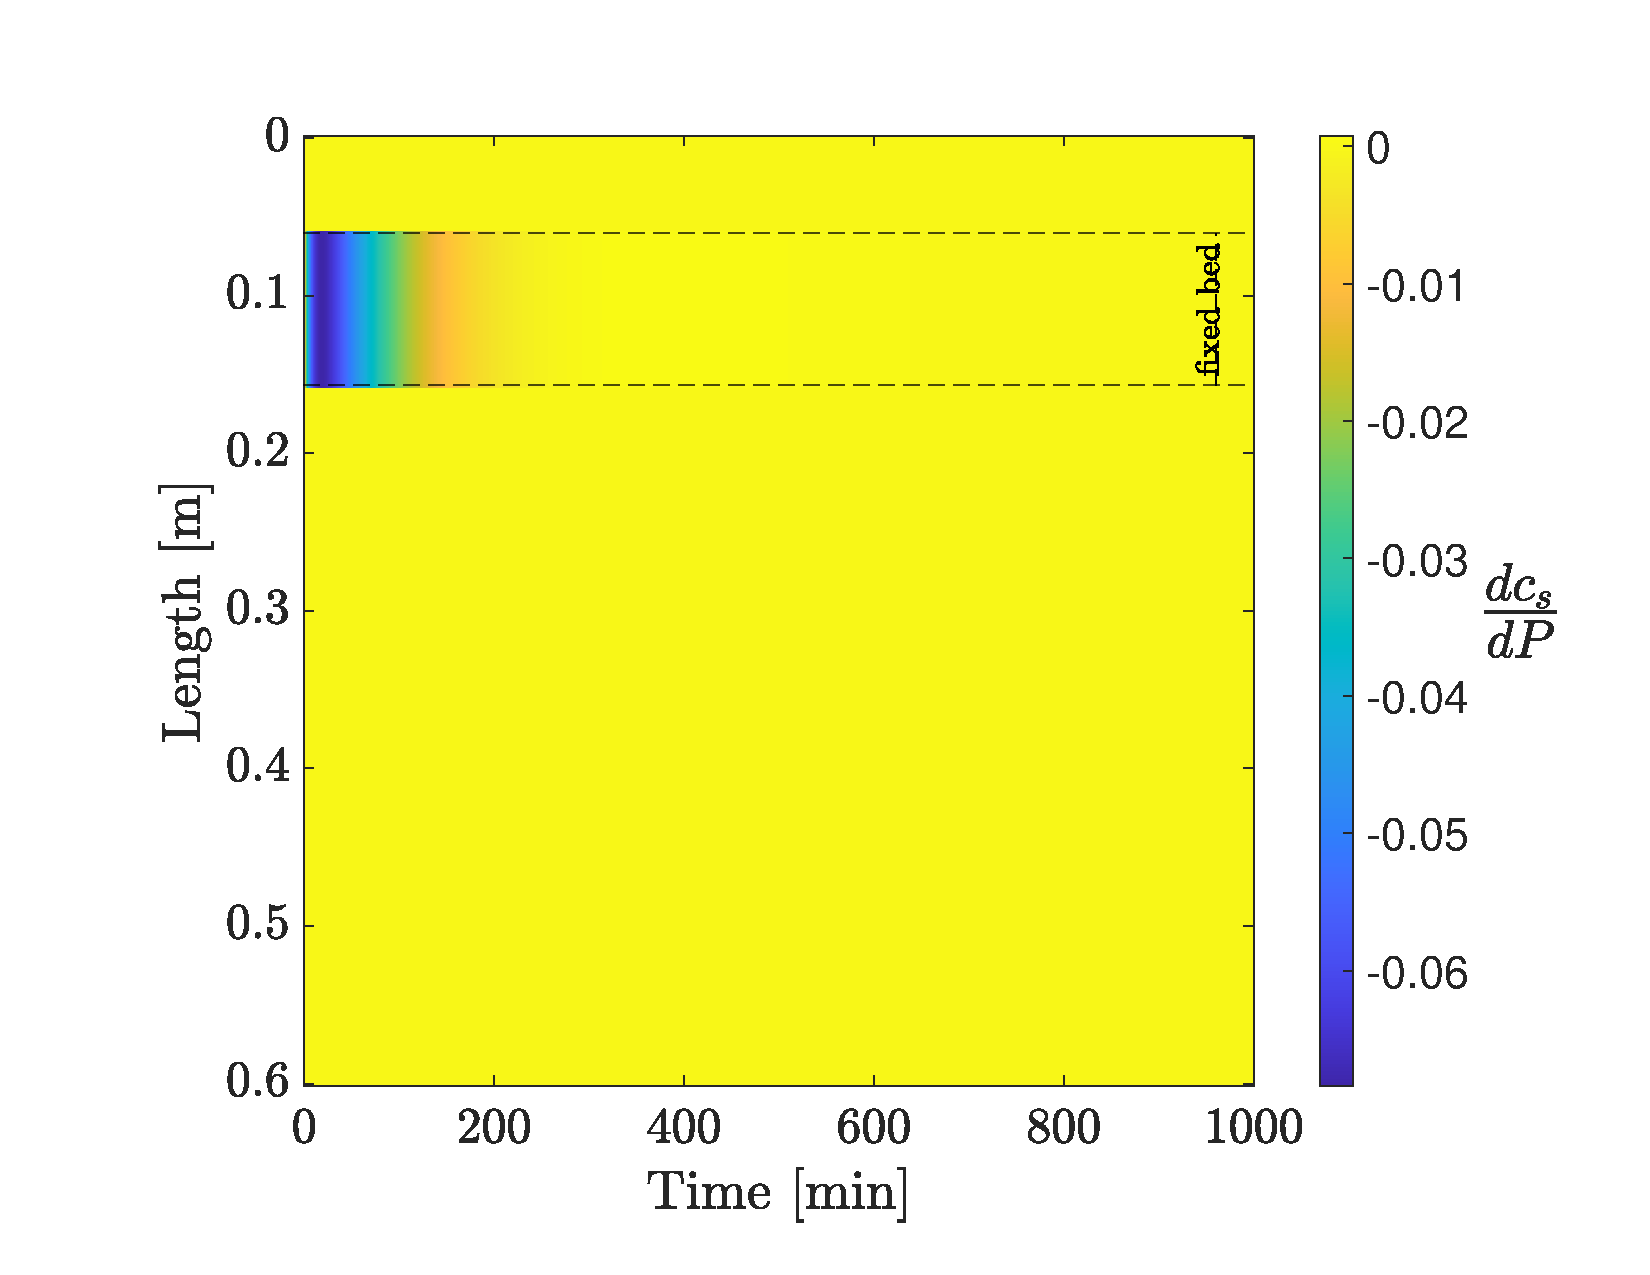
\includegraphics[trim = 1.5cm 1cm 0.0cm 1.0cm,clip,width=\columnwidth]{/Results_sensitivity/CS_P.pdf}
		\caption{The effect of $P$ change on $C_s$}
		\label{fig:Sensitivty_P_CS}
	\end{figure}

	The corresponding response of the pressure change on the solute concentration in the fluid phase is presented in Figure \ref{fig:Sensitivty_P_CF}. As discussed earlier, the pressure change directly influences the extraction kinetics. Figure \ref{fig:Sensitivty_P_CS} is characterized by negative sensitivities, suggesting a higher extraction rate due to the pressure change. Consequently, an increase in solute concentration in the fluid phase is expected. This increase in solute concentration in the fluid phase is visible in Figure \ref{fig:Sensitivty_P_CF} as positive sensitivities, forming a front that moves along the extractor. As the extraction process accelerates, more solute enters the fluid phase, explaining the "hot spot" in the Figure. Subsequently, the solute flows through the system where there are no solid particles, and the diffusion effect becomes noticeable. Following the positive sensitivities, a small front of negative sensitivities can be observed. Due to the higher extraction rate, more solute has been extracted at the beginning of the extraction process, resulting in less solute available for extraction later. This effect is reflected in Figure \ref{fig:Sensitivty_P_CF} as negative sensitivities. Eventually, the negative sensitivities approach zero.

	\begin{figure}[h!]
		\centering
		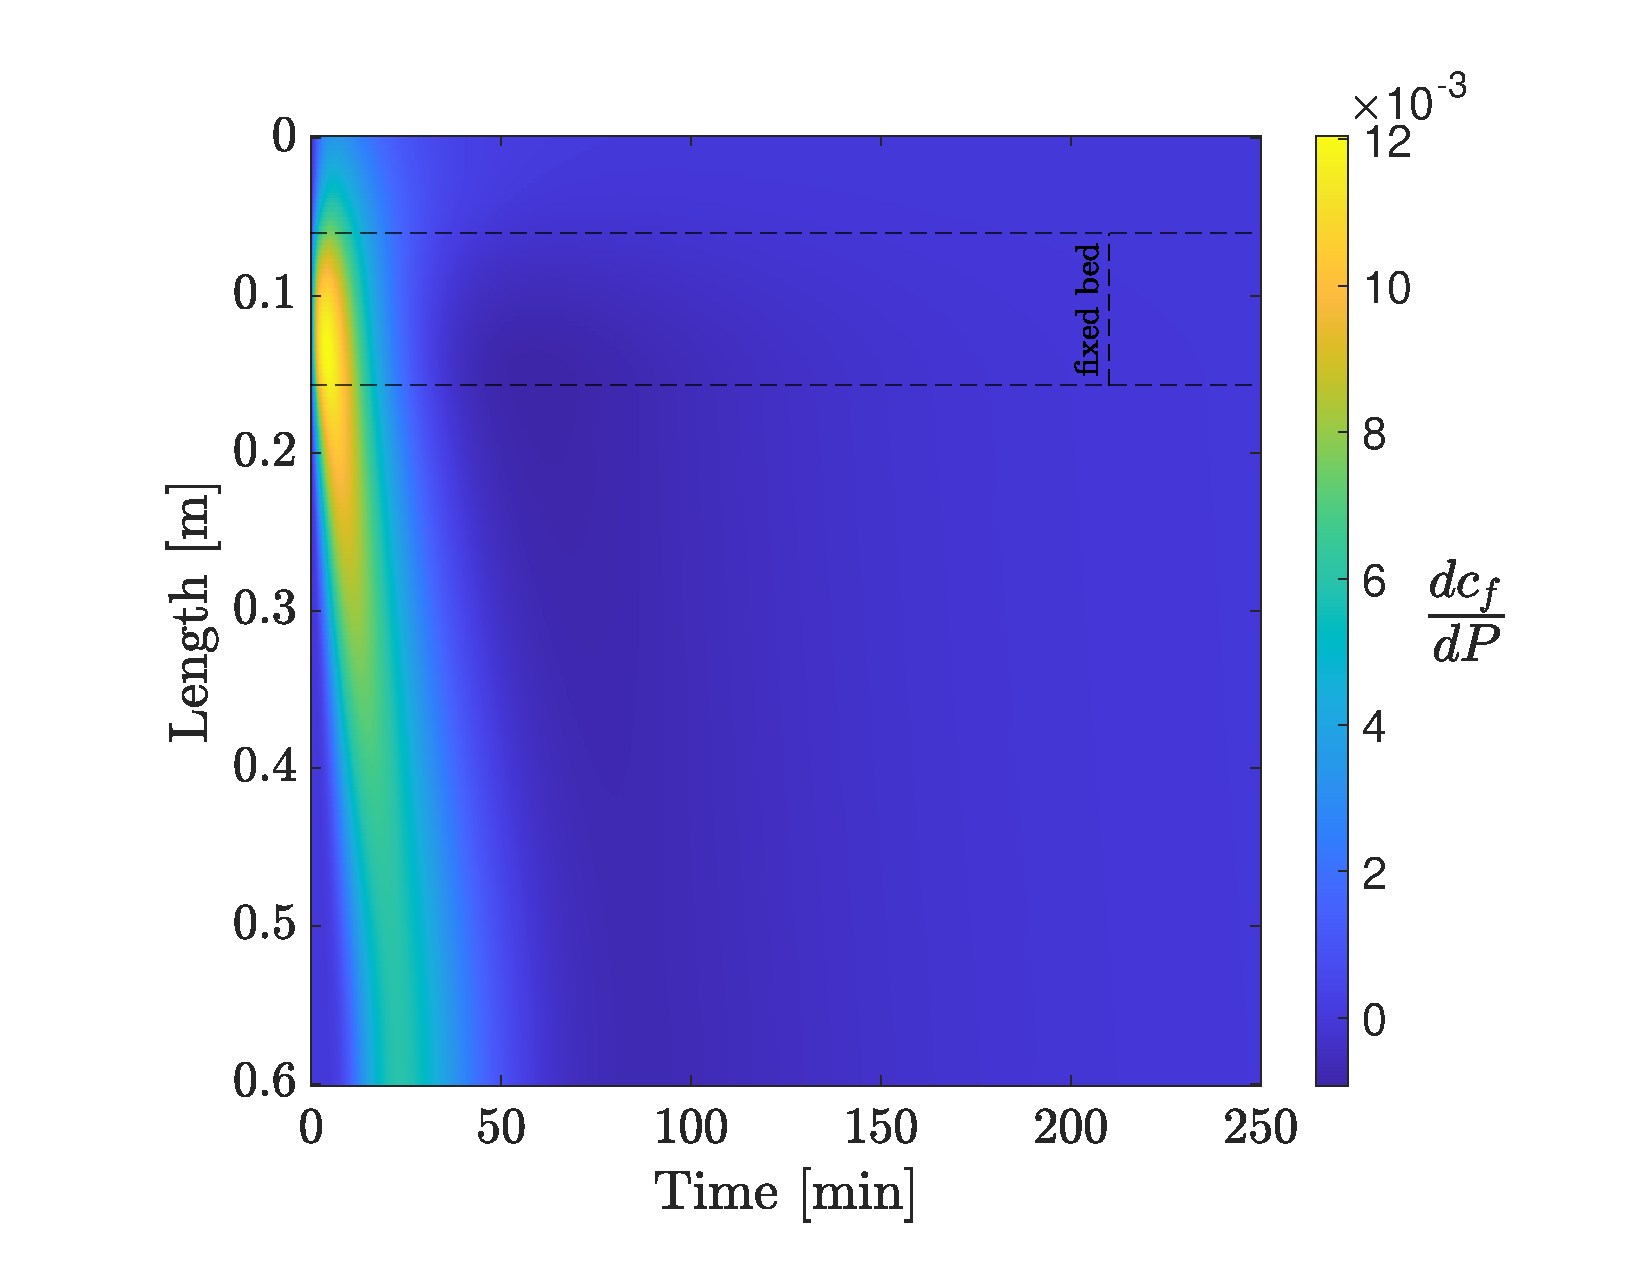
\includegraphics[trim = 1.5cm 1cm 0.0cm 1.0cm,clip,width=\columnwidth]{/Results_sensitivity/CF_P.pdf}
		\caption{The effect of $P$ change on $C_f$}
		\label{fig:Sensitivty_P_CF}
	\end{figure}

	The impact of pressure increase on extraction yield is depicted in Figure \ref{fig:Sensitivty_P_y}. The initial flat curve reflects a system delay, caused by the empty space within the extractor that the solvent with solute must traverse to reach the outlet. Next, a positive sensitivity starts to rise, which indicates an increase in yield. $dy / dP$ reaches its maximum and then declines due to a lower amount of solute remaining in the solid phase compared to the initial pressure conditions. This sensitivity eventually dips into negative values, hits a minimum point, and ultimately converges to zero. The simulation duration was extended to demonstrate the convergence of $dy / dP$ towards zero.

	\begin{figure}[h!]
		\centering
		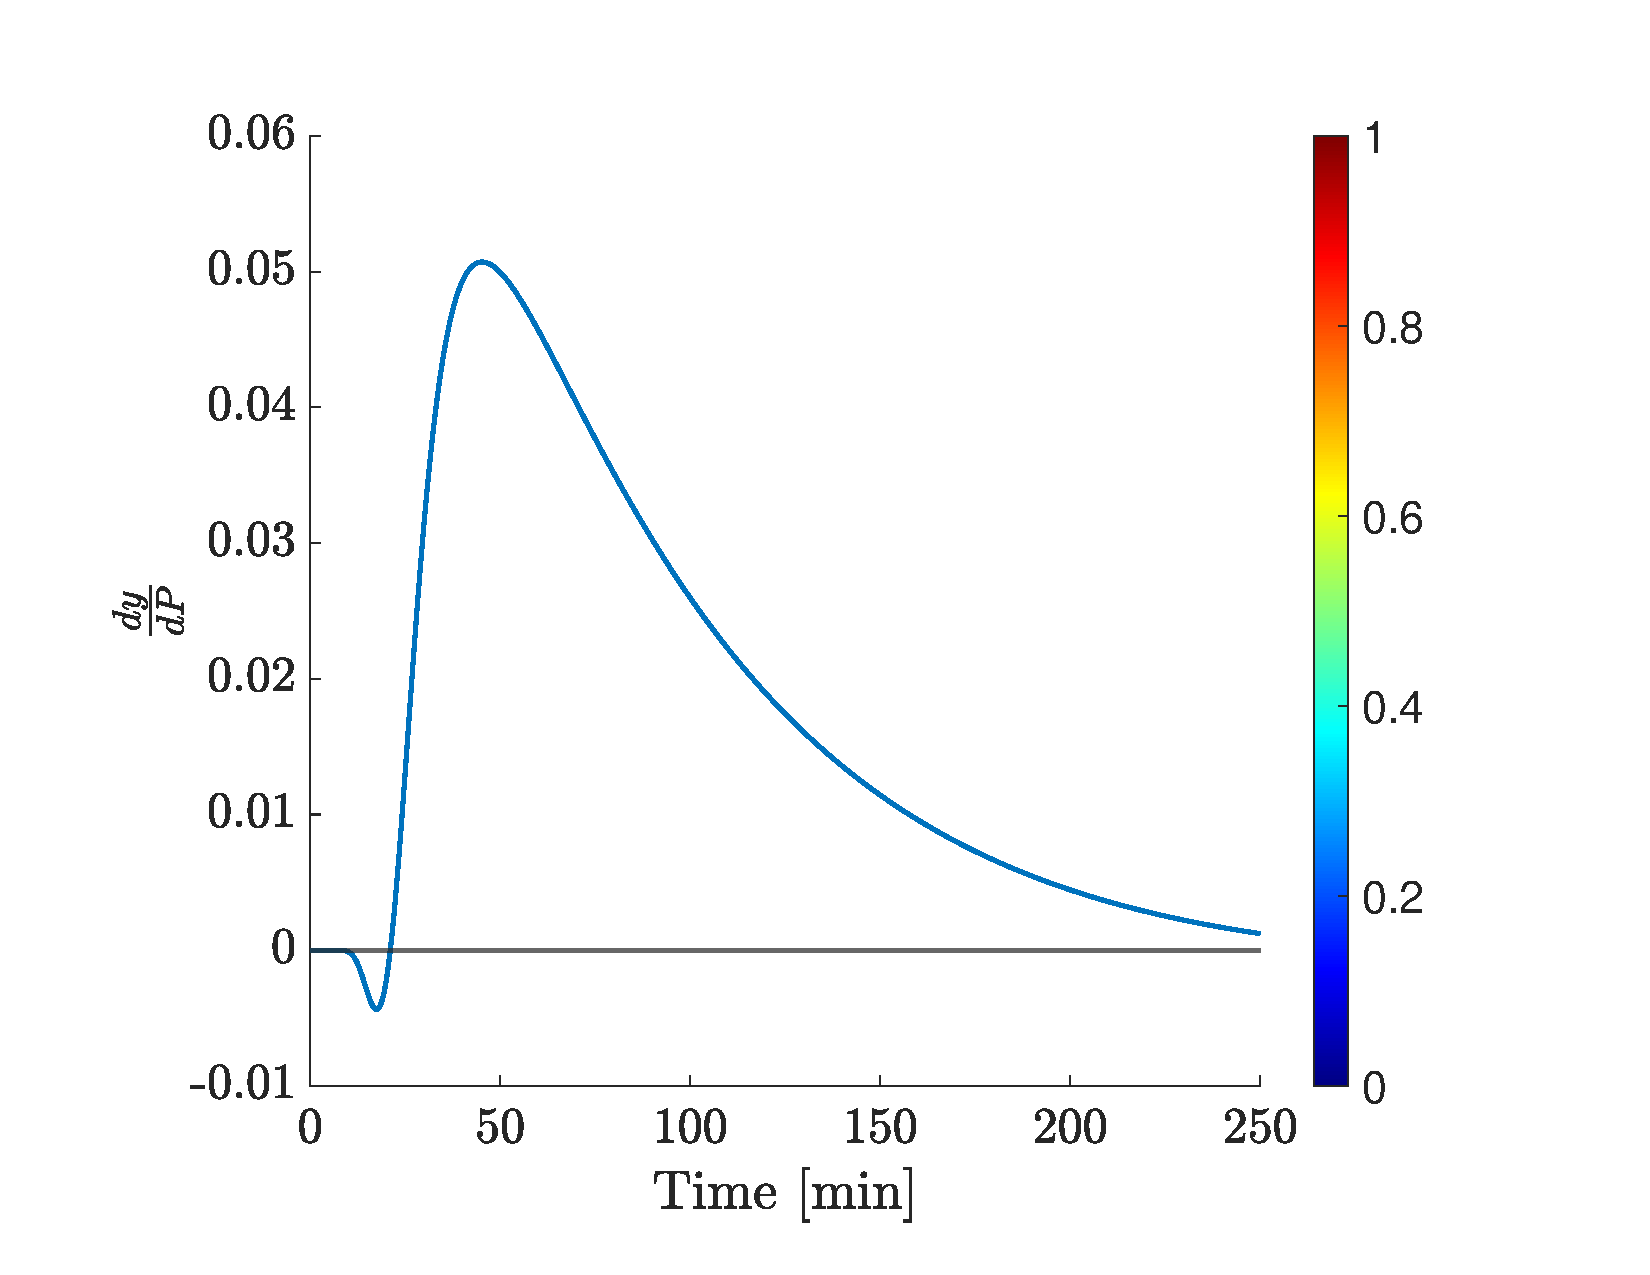
\includegraphics[trim = 1.5cm 1cm 0.0cm 1.0cm,clip,width=\columnwidth]{/Results_sensitivity/Y_P.pdf}
		\caption{The effect of $P$ change on $y(t)$}
		\label{fig:Sensitivty_P_y}
	\end{figure}

	\subsection{Inlet temperature}
	
	The impact of the inlet temperature on supercritical extraction differs from the two cases presented earlier because the disturbance does not instantaneously affect the entire system; instead, it propagates through the system. As the fluid with the modified temperature flows along the system, it gradually influences the mass transfer parameters. One important assumption is that the inlet temperature does not affect the pressure, and as a result, a horizontal line is present in Figure \ref{fig:Sensitivty_P_T}.
	
	\begin{figure}[h!]
		\centering
		\includegraphics[trim = 1.5cm 1cm 0.0cm 1.0cm,clip,width=\columnwidth]{/Results_sensitivity/P_T_{in}.pdf}
		\caption{The effect of $T_{in}$ change on $P$ in the system}
		\label{fig:Sensitivty_P_T}
	\end{figure}

	The propagation of the heat front is presented in Figure \ref{fig:Sensitivty_T_H}. Initially, the system was uniformly set to the same temperature. The temperatures at the inlet and outlet boundaries are predefined (Dirichlet boundary conditions) and consistent with those inside the system. The inlet value of $(h\times \rho_f)$ is calculated based on the provided inlet temperature and given pressure.  Any deviation in $T_{in}$ affects $(h\times \rho_f)$ at the inlet, which subsequently propagates according to the governing equations.
	
	\begin{figure}[h!]
		\centering
		\includegraphics[trim = 1.5cm 1cm 0.0cm 1.0cm,clip,width=\columnwidth]{/Results_sensitivity/H_T_{in}.pdf}
		\caption{The effect of $T_{in}$ change on $(h \times \rho_f)$ in the system}
		\label{fig:Sensitivty_T_H}
	\end{figure}

	Figure \ref{fig:Sensitivty_T_CS} illustrates how the change in inlet temperature affects the concentration of solute in the solid phase. Initially, the sensitivities are zero along the fixed bed because the heat front requires time to propagate to the fixed bed. Since this propagation is not instantaneous, a non-uniform distribution of sensitivities along the fixed bed becomes evident. All the sensitivities gradually increase until they reach their respective maxima. As presented in {\color{red}article 1}, the value of $D_i^R$ decreases as density decreases. Therefore, it is expected to observe positive sensitivities in Figure \ref{fig:Sensitivty_T_CS}, indicating a slower extraction rate. When the concentration gradient becomes the limiting factor, the sensitivities start to decrease to zero.

	\begin{figure}[h!]
		\centering
		\includegraphics[trim = 1.5cm 1cm 0.0cm 1.0cm,clip,width=\columnwidth]{/Results_sensitivity/CS_T_{in}.pdf}
		\caption{The effect of $T_{in}$ change on $C_s$ in the system}
		\label{fig:Sensitivty_T_CS}
	\end{figure}

	The influence of inlet temperature on solute concentration in the fluid phase is depicted in Figure \ref{fig:Sensitivty_T_CF}. Initially, all the sensitivities remain at zero due to an idle period. When the fluid at the new temperature reaches the solid particles, it affects mass transfer, subsequently influencing the amount of solute in the fluid phase. In response to the slower extraction rate indicated by positive sensitivities in Figure \ref{fig:Sensitivty_T_CS}, a section with negative sensitivities becomes visible in Figure \ref{fig:Sensitivty_T_CF}. The effect of diffusion is observable in the section without the fixed bed, where the front composed of sensitivities becomes blurred. After reaching their minima, the sensitivities increase and attain positive values. This behavior can be explained by considering that the heat front slowed mass transfer, causing more solute to remain in the solid phase. This, in turn, leads to a higher concentration gradient in the later stages of extraction compared to the scenario without the inlet temperature deviation. The higher concentration gradient results in an increase in $dc_f/dT_{in}$. 
	
	\begin{figure}[h!]
		\centering
		\includegraphics[trim = 1.5cm 1cm 0.0cm 1.0cm,clip,width=\columnwidth]{/Results_sensitivity/CF_T_{in}.pdf}
		\caption{The effect of $T_{in}$ change on $C_f$ in the system}
		\label{fig:Sensitivty_T_CF}
	\end{figure}

	Figure \ref{fig:Sensitivty_T_y} depicts how an increase in inlet temperature alters the extraction yield. Initially, the sensitivity curve remains flat. It is because the fixed bed doesn't occupy the entire volume of the extractor and the fluid requires some time to flow through the empty portion of the extractor to reach its outlet. It's only when the solute in the fluid phase reaches the extractor's outlet a system response can be observed. At this point, $dy/dT_{in}$ begins to decrease, and the negative sensitivity value indicates a decrease in process efficiency. Over time, the sensitivity reaches its minimum and then increases due to a higher concentration gradient compared to the case without the disturbance. The sensitivity reaches a positive maximum and then declines again due to reduced extraction kinetics and a decreased concentration gradient. $dy/dT_{in}$ becomes negative once more, eventually resulting in a flattening of the sensitivity curve. The flattening of the yield curve suggest that the mass transfer parameters limits the extraction rate and the residual solute in the solid phase become difficult to obtain.

	\begin{figure}[h!]
		\centering
		\includegraphics[trim = 1.5cm 1cm 0.0cm 1.0cm,clip,width=\columnwidth]{/Results_sensitivity/Y_T_{in}.pdf}
		\caption{The effect of $T_{in}$ change on $y(t)$ in the system}
		\label{fig:Sensitivty_T_y}
	\end{figure}
	
\end{document}


































